\chapter{Instalasi dan Konfigurasi \textbf{\textit{Python}}}

\section{Instalasi \textbf{\textit{Python}}}
Untuk instalasi python pada Ubuntu 19.04 dibutuhkan sebagai berikut:

\begin{enumerate}
\item Internet
\item Anaconda installer (64bit or 32bit)
\item enter, dan yes atau no
\end{enumerate}

Ikuti langkah berikut:
\begin{enumerate}
\item Pertama kita kunjungi situs \textbf{\textit{https://www.anaconda.com/distribution/\#download-section}} seperti gambar ~\ref{anacondadownload} dan pilih \textbf{64-Bit (x86) Installer (517 MB)}
\begin{figure}[H]
\centering
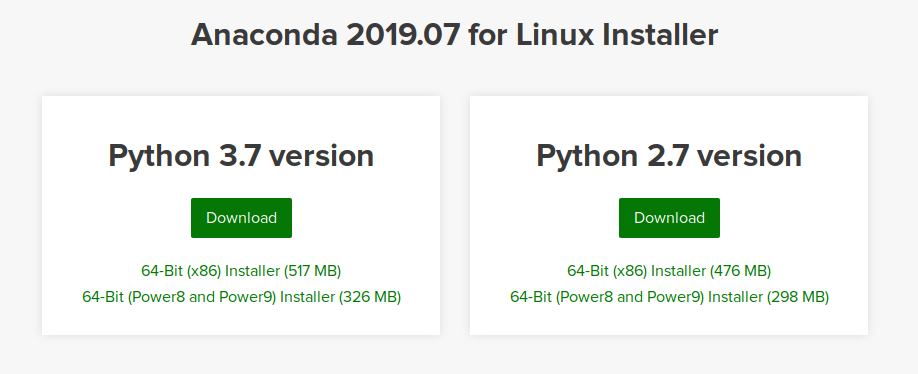
\includegraphics[width=1\textwidth]{figures/anacondadownload.png}
\caption{Gambar halaman download}
\label{anacondadownload}
\end{figure}

\item Kedua kita buka \textit{\textbf{terminal}} kita lalu arahkan ke direktori kita menyimpan file download anaconda

\item Ketiga kita ketikkan sebagai berikut \textbf{bash \textit{namafileanaconda}.sh} lalu enter, contoh seberti gambar \ref{anacondabash}
\begin{figure}[H]
\centering
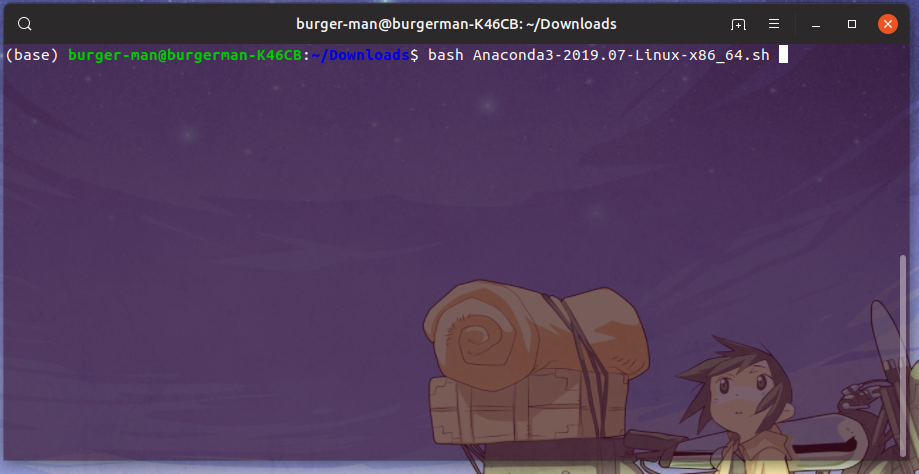
\includegraphics[width=1\textwidth]{figures/anacondabash.png}
\caption{Gambar install anaconda}
\label{anacondabash}
\end{figure}

\item Setelah itu, tekan \textbf{ENTER} saja seperti gambar \ref{anacondaenter}
\begin{figure}[H]
\centering
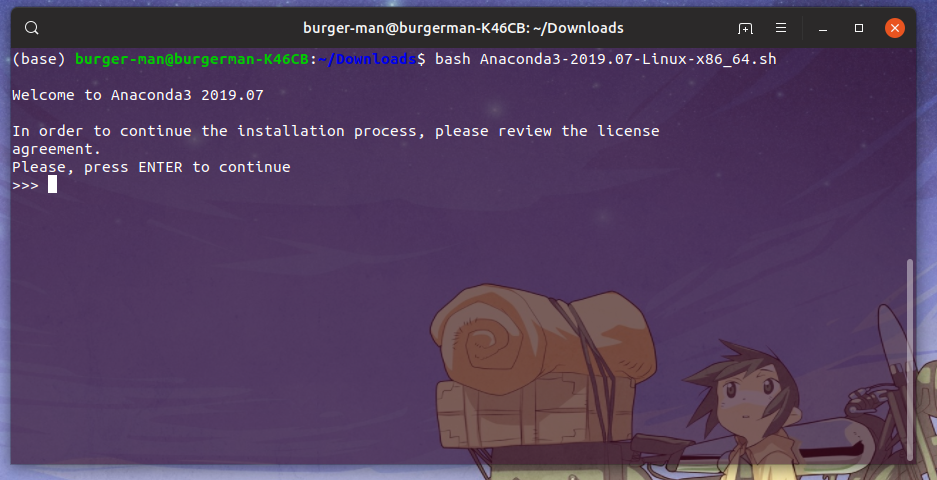
\includegraphics[width=1\textwidth]{figures/anacondaenter.png}
\caption{Gambar eksekusi anaconda}
\label{anacondaenter}
\end{figure}

\item Lalu akan muncul sebuah tulisan \textbf{End User License Agreement} seperti gambar \ref{entertrus}, tekan \textbf{ENTER} dan tahan hingga seperti gambar 
\begin{figure}[H]
\centering
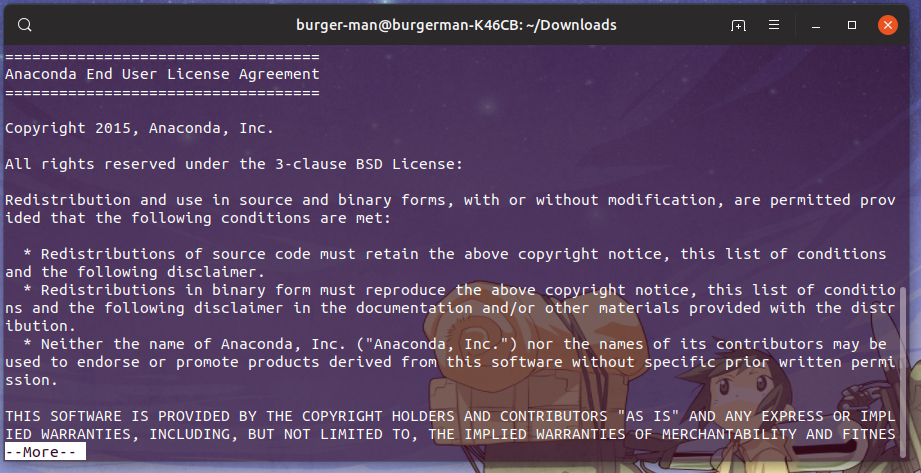
\includegraphics[width=1\textwidth]{figures/entertrus.png}
\caption{Gambar anaconda license agreement}
\label{entertrus}
\end{figure}
\begin{figure}[H]
\centering
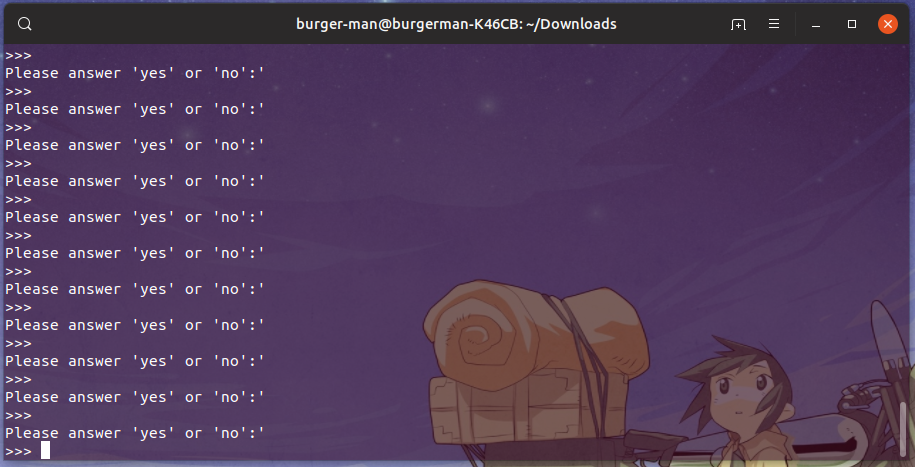
\includegraphics[width=1\textwidth]{figures/enterkekgini.png}
\caption{Gambar perintah yes or no}
\label{enterkekgini}
\end{figure}

\item Lalu setelah muncur perintah \textbf{\textit{'yes' or 'no'}} ketik \textbf{\textit{yes}} lalu enter

\item Setelah itu muncul path direktori instalasi anaconda kita seperti gambar \ref{enterpath} lalu tekan enter
\begin{figure}[H]
\centering
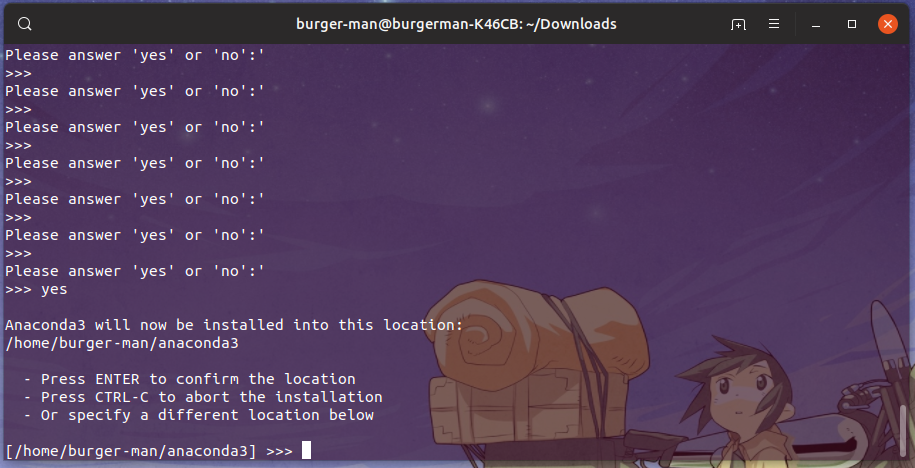
\includegraphics[width=1\textwidth]{figures/enterpath.png}
\caption{Gambar path anaconda}
\label{enterpath}
\end{figure}

Setelah kita selesai instalasi anaconda jangan lupa juga untuk menginstal spyder ide, caranya seperti berikut:
\begin{enumerate}

\item ketikkan perintah \textbf{\textit{sudo apt install spyder3 -y}} seperti gambar \ref{installspyder3}
\begin{figure}[H]
\centering
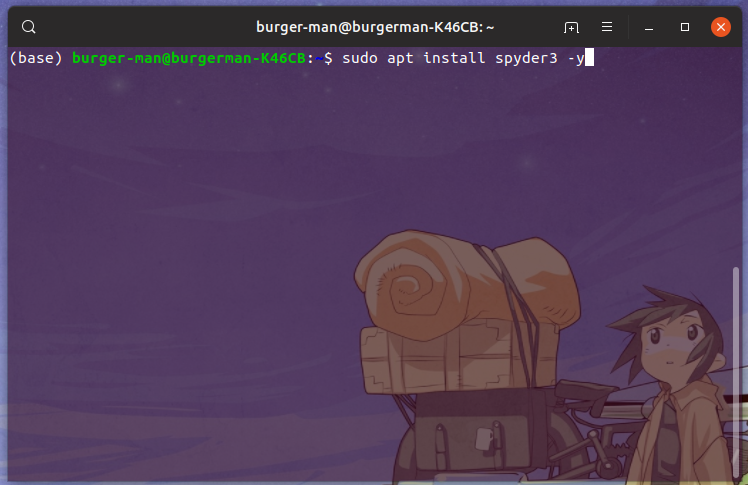
\includegraphics[width=1\textwidth]{figures/installspyder3.png}
\caption{Gambar perintah install spyder3}
\label{installspyder3}
\end{figure}

\item lalu jalankan dengan perintah \textbf{\textit{spyder}} atau \textbf{\textit{spyder3}}
\end{enumerate}

\end{enumerate}

\section{Konfigurasi \textbf{\textit{Python}}}
Setelah kita selesai instal Anaconda dan Spyder, selanjutnya kita akan mempelajari bagaimana cara setting environments python kita? caranya sebagai berikut

\begin{enumerate}

\item pertama kita buka terminal kita lalu ketikkan perintah \textbf{export PYTHONPATH=\$PYTHONPATH:\textit{pathinstallasipythonkalian}} contoh seperti gambar \ref{setpath}, lalu enter
\begin{figure}[H]
\centering
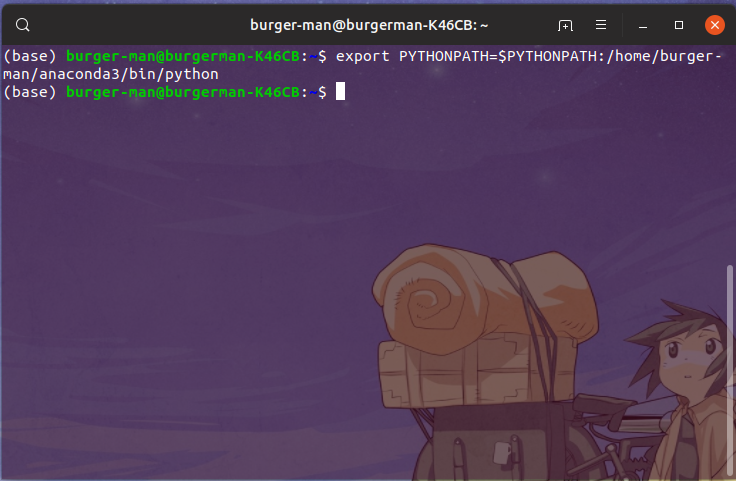
\includegraphics[width=1\textwidth]{figures/setpath.png}
\caption{Gambar setpath}
\label{setpath}
\end{figure}

\end{enumerate}

\section{Instalasi \textbf{\textit{pip}}}
Apa itu pip? pip adalah sebuah standard package atau sebuah perintah yang digunakan untuk menginstal seluruh kebutuhan package yang akan digunakan, caranya sebagai berikut

\begin{enumerate}

\item pertama kita buka terminal kita lalu ketikkan perintah \textbf{sudo apt install python3-pip -y} untuk pip3 dan \textbf{sudo apt install python2-pip -y} untuk pip2 contoh seperti gambar \ref{installpip}, lalu enter
\begin{figure}[H]
\centering
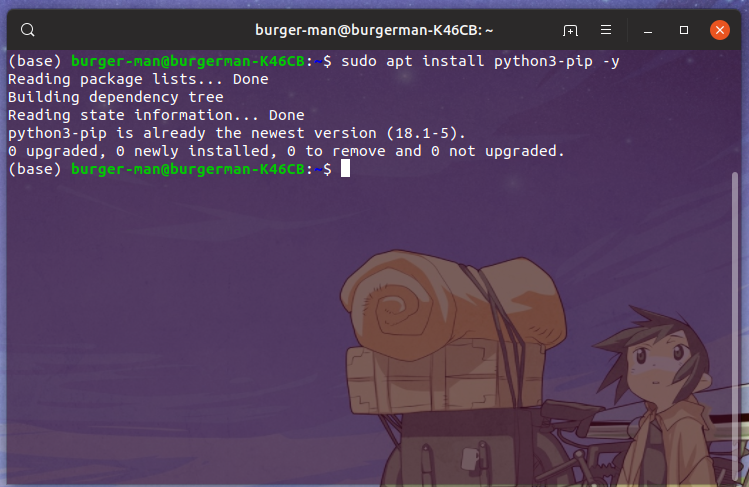
\includegraphics[width=1\textwidth]{figures/installpip.png}
\caption{Gambar instal pip}
\label{installpip}
\end{figure}

\end{enumerate}

\section{Update anaconda dan spyder}
Kadang kala anaconda dan spyder melakukan update software terbaru, lalu bagaimana caranya update software tanpa uninstall? berikut caranya

\begin{enumerate}
\item Pertama buka terminal dan ketikkan \textbf{\textit{conda update --all}} seperti gambar \ref{condauptade}, lalu enter
\begin{figure}[H]
\centering
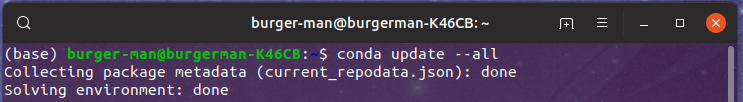
\includegraphics[width=1\textwidth]{figures/updateconda.png}
\caption{Gambar update anaconda}
\label{updateconda}
\end{figure}

\item Tunggu proses berjalan hingga muncul seperti gambar \ref{pressy}, lalu ketik \textbf{\textit{y}} lalu enter
\begin{figure}[H]
\centering
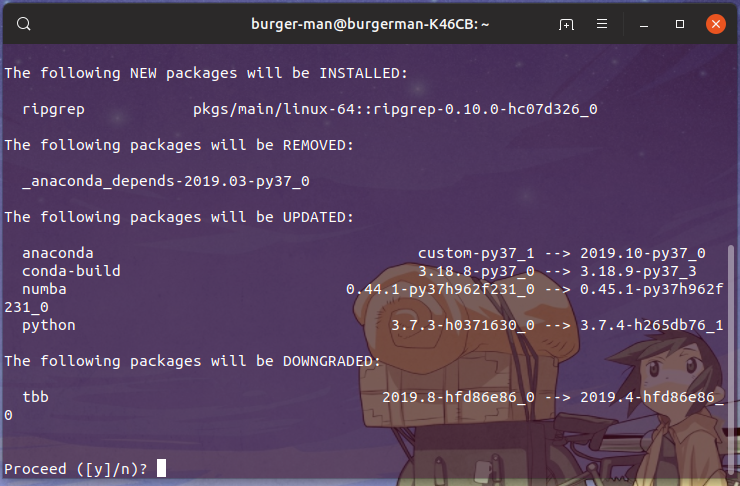
\includegraphics[width=1\textwidth]{figures/pressy.png}
\caption{Gambar update anaconda}
\label{pressy}
\end{figure}

\item Lalu tunggu hingga proses download dan instalasi selesai
\end{enumerate}

Update Spyder:
Ada dua cara untuk update spyder yaitu dengan pip atau dengan conda, kali ini saya memakai anaconda sebagai perantara update spyder, sebagai berikut

\begin{enumerate}
\item Pertama buka terminal dan ketikkan \textbf{\textit{conda update spyder}} seperti gambar \ref{updatespyder}, lalu enter
\begin{figure}[H]
\centering
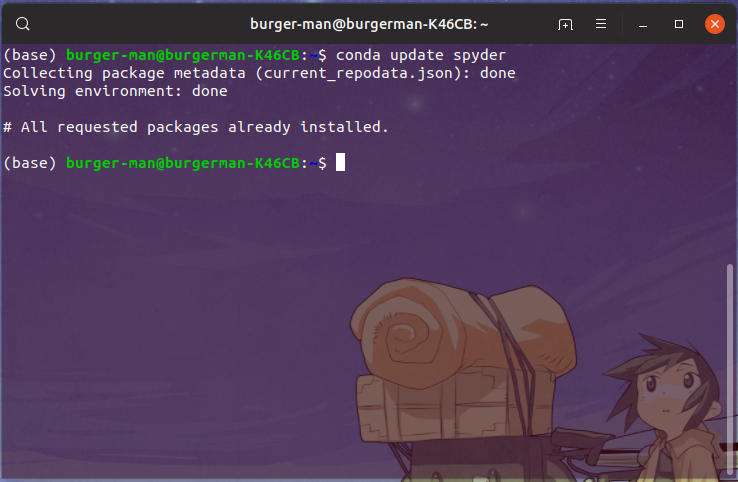
\includegraphics[width=1\textwidth]{figures/updatespyder.png}
\caption{Gambar update spyder}
\label{updatespyder}
\end{figure}

\item Dalam kasus ini spyder saya sudah up-to-date sehingga tidak ada update dari spyder, jikalau ada, maka tinggal ketik \textbf{\textit{y}} lalu enter dan tunggu hingga proses download dan instalasi selesai
\end{enumerate}